\section{参数的梯度更新}
\label{sec:dapx-gradient}

逐因子更新依赖一个前提：每个因子可以是任意分布，于是“取指数再归一化”的结果总在候选集合里。若要求因子属于某个参数族，比如规定每个因子都是高斯分布，而目标不是高斯分布，式~\eqref{eq:dapx-cavi-update}给出的$\exp(g_j)$一般不再是高斯密度，更新会跳出候选集合。又比如章首的四次方目标只有一个变量，没有可以拆分的因子。这时候选集合是一个有限维参数族，逼近问题就成了参数的优化问题。

\paragraph{参数优化问题}
设候选集合为$\{Q_{\bm{\theta}}:\bm{\theta}\in\Theta\}$，$\Theta\subset\mathbb{R}^{d}$是开集，密度$q_{\bm{\theta}}$对$\bm{\theta}$可微。按候选加权的方向，由式~\eqref{eq:dapx-J}，要最小化
\begin{equation}
 J(\bm{\theta})=\mathbb{E}_{Q_{\bm{\theta}}}\bigl[\ln q_{\bm{\theta}}(X)-\ln\widetilde{\pi}(X)\bigr] .
 \label{eq:dapx-J-theta}
\end{equation}
按目标加权的方向，在式~\eqref{eq:dapx-forward-split}成立的范围内，要最小化$-\mathbb{E}_{\Pi}[\ln q_{\bm{\theta}}(X)]$。只要目标函数可微，就可以用\BookChapterRef{chap:first-order-methods}{卷五第6章“一阶方法”}的梯度下降，
\begin{equation}
 \bm{\theta}^{(t+1)}=\bm{\theta}^{(t)}-\eta\,\nabla J\bigl(\bm{\theta}^{(t)}\bigr) ,
 \label{eq:dapx-gd}
\end{equation}
其中$\eta>0$是步长。参数还可以与乘积结构结合：每个因子取一个参数族，对所有因子的参数一起做梯度更新，或者在没有闭式解的那些因子上用梯度步代替式~\eqref{eq:dapx-cavi-update}。

两个方向的梯度对计算的要求不同。按目标加权时，在求导与期望可以交换的条件下，
\[
 \nabla_{\bm{\theta}}\bigl(-\mathbb{E}_{\Pi}[\ln q_{\bm{\theta}}(X)]\bigr)=-\mathbb{E}_{\Pi}\bigl[\nabla_{\bm{\theta}}\ln q_{\bm{\theta}}(X)\bigr] ,
\]
期望仍按目标计算；对指数族它就是$\nabla A(\bm{\theta})-\mathbb{E}_{\Pi}[\bm{T}]$，零点正是定理~\ref{thm:dapx-moment-matching}的矩匹配。按候选加权时，被积函数和求期望的分布都依赖$\bm{\theta}$，求导要同时处理两处。本节的例子里期望有闭式，可以直接求导；没有闭式时，要用样本构造梯度的随机估计，什么时候能交换求导与期望、怎样构造方差小的估计，是第~\ref{chap:expectation-gradient-estimation}章的内容，有了随机梯度后的迭代方法见\BookChapterRef{chap:stochastic-gradient-methods}{卷五第13章“随机梯度方法”}。

\paragraph{按目标加权：指数族上的凸问题}
候选是指数族时，按目标加权的目标函数在自然参数下是凸的。在式~\eqref{eq:dapx-forward-split}成立的范围内，与$\bm{\theta}$有关的部分是
\[
 -\mathbb{E}_{\Pi}[\ln q_{\bm{\theta}}(X)]=A(\bm{\theta})-\langle\bm{\theta},\mathbb{E}_{\Pi}[\bm{T}]\rangle-\mathbb{E}_{\Pi}[\ln h(X)] .
\]
第~\ref{chap:distribution-families}章证明了$A$的Hessian是$\bm{T}$的协方差矩阵，半正定，所以$A$是凸函数，再减去一个线性函数仍是凸的。凸函数的驻点就是全局最小点，梯度下降不会停在别处。

用三状态例子走几步。$Q_t$的自然参数$\theta$满足$t=\mathrm{e}^{\theta}/(1+2\mathrm{e}^{\theta})$，对数配分函数$A(\theta)=\ln(1+2\mathrm{e}^{\theta})$，$A'(\theta)=2t$，所以梯度就是矩的差：
\[
 \frac{\mathrm{d}}{\mathrm{d}\theta}D_{\mathrm{KL}}(\Pi\Vert Q_t)=2t-0.7 .
\]
取步长$\eta=2$，从$\theta^{(0)}=0$即$t=\tfrac13$出发。第一步的梯度是$\tfrac23-0.7=-0.0333$，于是
\[
 \theta^{(1)}=0+2\cdot0.0333=0.0667,\qquad t^{(1)}=0.3407 .
\]
第二步梯度为$-0.0187$，得到
\[
 \theta^{(2)}=0.104,\qquad t^{(2)}=0.3447 .
\]
在最优点附近，二阶导数$A''(\theta^{*})$等于$2t_{\mathrm{f}}(1-2t_{\mathrm{f}})=0.21$，梯度每步约乘以
\[
 1-\eta A''(\theta^{*})=1-2\cdot0.21=0.58 .
\]
第$7$步$t=0.3497$，趋于$t_{\mathrm{f}}=0.35$，对应$\theta^{*}=\ln(0.35/0.3)\approx0.154$。

按候选加权的目标函数没有这样的结构。它依赖$\bm{\theta}$的方式既通过$\ln q_{\bm{\theta}}$，也通过求期望的分布本身，在自然参数下一般不是凸的：第~\ref{sec:dapx-direction-compare}节双峰目标上的两个局部最小点就是例子。所以按候选加权时，梯度下降的结果要结合初值来解释。

\paragraph{参数化保持合法}
梯度步是在$\mathbb{R}^{d}$里走一步，走完后的参数必须仍然对应一个合法的分布。对四次方目标取候选$\mathcal{N}(m,s^{2})$，若直接以$(m,s)$为参数，由式~\eqref{eq:dapx-quartic-J}，
\[
 \frac{\partial J}{\partial s}=-\frac1s+3m^{2}s+3s^{3} .
\]
在$m=0$、$s=1.5$处它等于$-0.667+10.125=9.458$，取步长$\eta=0.2$，一步后$s=1.5-1.892<0$，不再是标准差。

改用$\omega=\ln s$作参数，$s=\mathrm{e}^{\omega}$对任何实数$\omega$都是正的，约束自动满足。由链式法则，
\[
 \frac{\partial J}{\partial\omega}=s\,\frac{\partial J}{\partial s}=1.5\cdot9.458=14.19 .
\]
同样的步长下，一步后
\[
 \omega=\ln1.5-0.2\cdot14.19=-2.43,\qquad s=\mathrm{e}^{-2.43}\approx0.088 .
\]
这个$s$合法，却走得太远，说明步长仍要另行选择；重新参数化只解决合法性。同样的办法用于其他约束：概率向量写成$p_k=\mathrm{e}^{u_k}/\sum_l\mathrm{e}^{u_l}$；协方差矩阵写成$\bm{L}\bm{L}^{\top}$，$\bm{L}$是对角元取指数的下三角矩阵，于是总是对称正定。

\paragraph{四次方目标的梯度下降}
以$(m,\omega)$为参数，把$s=\mathrm{e}^{\omega}$代入式~\eqref{eq:dapx-quartic-J}：
\[
 J(m,\omega)=-\omega-C+\tfrac14\bigl(m^{4}+6m^{2}\mathrm{e}^{2\omega}+3\mathrm{e}^{4\omega}\bigr) .
\]
分别求偏导，得到
\begin{equation}
 \frac{\partial J}{\partial m}=m^{3}+3ms^{2},\qquad \frac{\partial J}{\partial\omega}=-1+3m^{2}s^{2}+3s^{4} .
 \label{eq:dapx-quartic-grad}
\end{equation}
梯度为零要求$m(m^{2}+3s^{2})=0$，即$m=0$，再由第二式得$s^{4}=\tfrac13$，与第~\ref{sec:dapx-reverse-kl}节的结果一致。

取$\eta=0.1$，从$(m,\omega)=(1,0)$即$\mathcal{N}(1,1)$出发。第一步的梯度由式~\eqref{eq:dapx-quartic-grad}算出：
\[
 \frac{\partial J}{\partial m}=1+3=4,\qquad \frac{\partial J}{\partial\omega}=-1+3+3=5 .
\]
由式~\eqref{eq:dapx-gd}，
\[
 m^{(1)}=1-0.4=0.6,\qquad \omega^{(1)}=0-0.5=-0.5,\qquad s^{(1)}=\mathrm{e}^{-0.5}\approx0.6065 .
\]
第二步$s^{2}\approx0.3679$，$s^{4}\approx0.1353$，梯度为
\[
 \begin{aligned}
 \frac{\partial J}{\partial m}&=0.216+3\cdot0.6\cdot0.3679=0.8782,\\
 \frac{\partial J}{\partial\omega}&=-1+3\cdot0.36\cdot0.3679+3\cdot0.1353=-0.1967 ,
 \end{aligned}
\]
于是$m^{(2)}=0.5122$，$\omega^{(2)}=-0.4803$。

用$D_{\mathrm{KL}}=J+\ln Z$记录离目标的远近，前几步依次为$2.022$、$0.355$、$0.280$；第$10$步为$0.0654$，第$20$步为$0.0476$，第$40$步与族内最小值$0.0472$相同到四位小数。图~\ref{fig:dapx-gradient-path}(a)中，第一步把$\omega$拉低了很多，此后路径沿着一条弯曲的谷慢慢移向最优点。

\begin{BookInlineFigure}
 \centering
 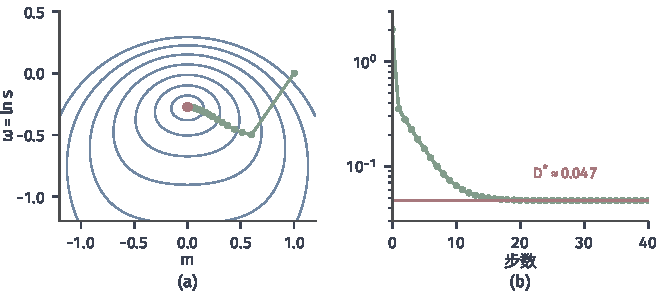
\includegraphics[width=112mm]{figures/07-probability/07-distribution-optimization/matplotlib/dapx-gradient-path/figure.pdf}
 \caption{四次方目标上高斯候选的梯度下降，参数$(m,\omega)$，$\omega=\ln s$，步长$0.1$。(a)$J(m,\omega)$的等高线（蓝）与$40$步的路径（绿），起点$(1,0)$，红点是最优解$(0,-\tfrac14\ln3)$。(b)各步的$D_{\mathrm{KL}}(Q^{(t)}\Vert\Pi)$（绿，对数纵轴），红线是族内最小值$0.0472$。}
 \label{fig:dapx-gradient-path}
\end{BookInlineFigure}

后期的收敛主要受$m$拖累。在最优点附近$s^{2}\approx3^{-1/2}$，$\partial J/\partial m\approx3s^{2}m\approx1.73\,m$，每步$m$乘以$1-0.173=0.827$，要把$m$从$0.1$降到$10^{-4}$约需$36$步。$\omega$方向的曲率不同，收敛快得多。各方向曲率不同时，同一个步长对某些方向太小、对另一些方向又可能太大，这是梯度下降在病态问题上的典型表现。在分布逼近中还有一层含义：参数空间里同样长的一步，在不同参数、不同位置引起的分布变化可能相差很大，$s$很小时改变$m$一点点，分布就几乎不再重叠。用分布本身的变化来度量步长、据此调整更新方向，是第~\ref{chap:information-geometry}章的内容。
